\section{Experimental Dataset}

\subsection{Mobile Phone Data Source}
\label{subsec:mobiledatasource}

The data used in this study consist of a set \( \mathP \) of \textit{Call Detail Records} (CDRs), composed of voice calls and text messages from a Mexican telecommunication company (\textit{telco}) for a 3 month period.

Every CDR \( p \in \mathP \) contains the phone numbers of the caller and callee \( \left< p_o, p_d \right> \), which are anonymized using a cryptographic hash function for privacy reasons, the starting time \( p_t \), and, in the case of voice calls, the call duration \( p_s \). The latitude and longitude of the antenna used for each call \( \left< p_y, p_x \right> \) are also given for a subset of the data.

Given that our collection \( \mathP \) of CDRs are coming from one telephone company, we are able to reconstruct all communication links between clients of this company, as well as communications between the clients and other users, but we have no information on communications where neither users are clients of our telco company.

If we define \( N \) as the set of clients of the telco, and \( \mathP_N \subseteq \mathP \) as the calls where \( \forall p \in \mathP_N, \; p_o \in N \wedge p_d \in N \), we create a communications graph \( \mathG_N \) which contains only the users from the telco, and all the calls exchanged between them.

\todo{Add data where we include the time and SMS (?) of each call.}

\todo{Explain telco vs non-telco}

\todo{Separate into $P$ for calls and $S$ for SMS}

%With the data provided to us by the telco, \( \mathG \) contains \num{72107108} users who made \num{72107108} calls and sent \num{634225740} text messages in this period of 3 months.

\subsection{Banking Information}

For this study we also used account balances for over 10 million clients of a bank in Mexico for a period of 6 months, denoted \( \mathB \). The data for each client \( b \in \mathB \) contains his phone number \( b_p \), anonymized with the same hash function used in \( \mathP \), and the reported income of this person over 6 months \( b_{s_0}, \ldots, b_{s_5} \). We average these 6 values to get \( b_s \), an estimate of a user's income.

The bank also provided us demographic information for a subset of its clients \( \mathA \subseteq \mathB \). For each user \( u \in \mathA \), we are given the age \( u_a \) of the user, which allows us to observe differences in the income distribution according to the age. In another line of work, homophily with respect to age has been observed and used to generate inferences~\cite{brea2014}.

\begin{figure}[h]
\begin{center}
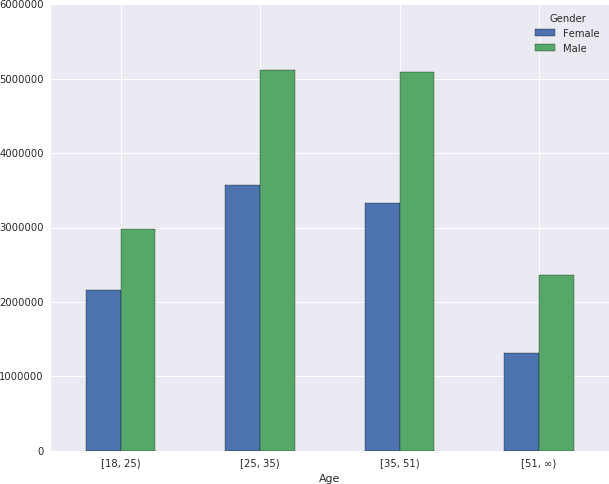
\includegraphics[width=0.9\columnwidth]{figures/gender_age_bar3/gender_age_bar3.png}
\caption{Amount of users in \( \mathB \) by gender and age.}
\label{gender_age_bar}
\end{center}
\end{figure}

\begin{figure}[h]
\begin{center}
{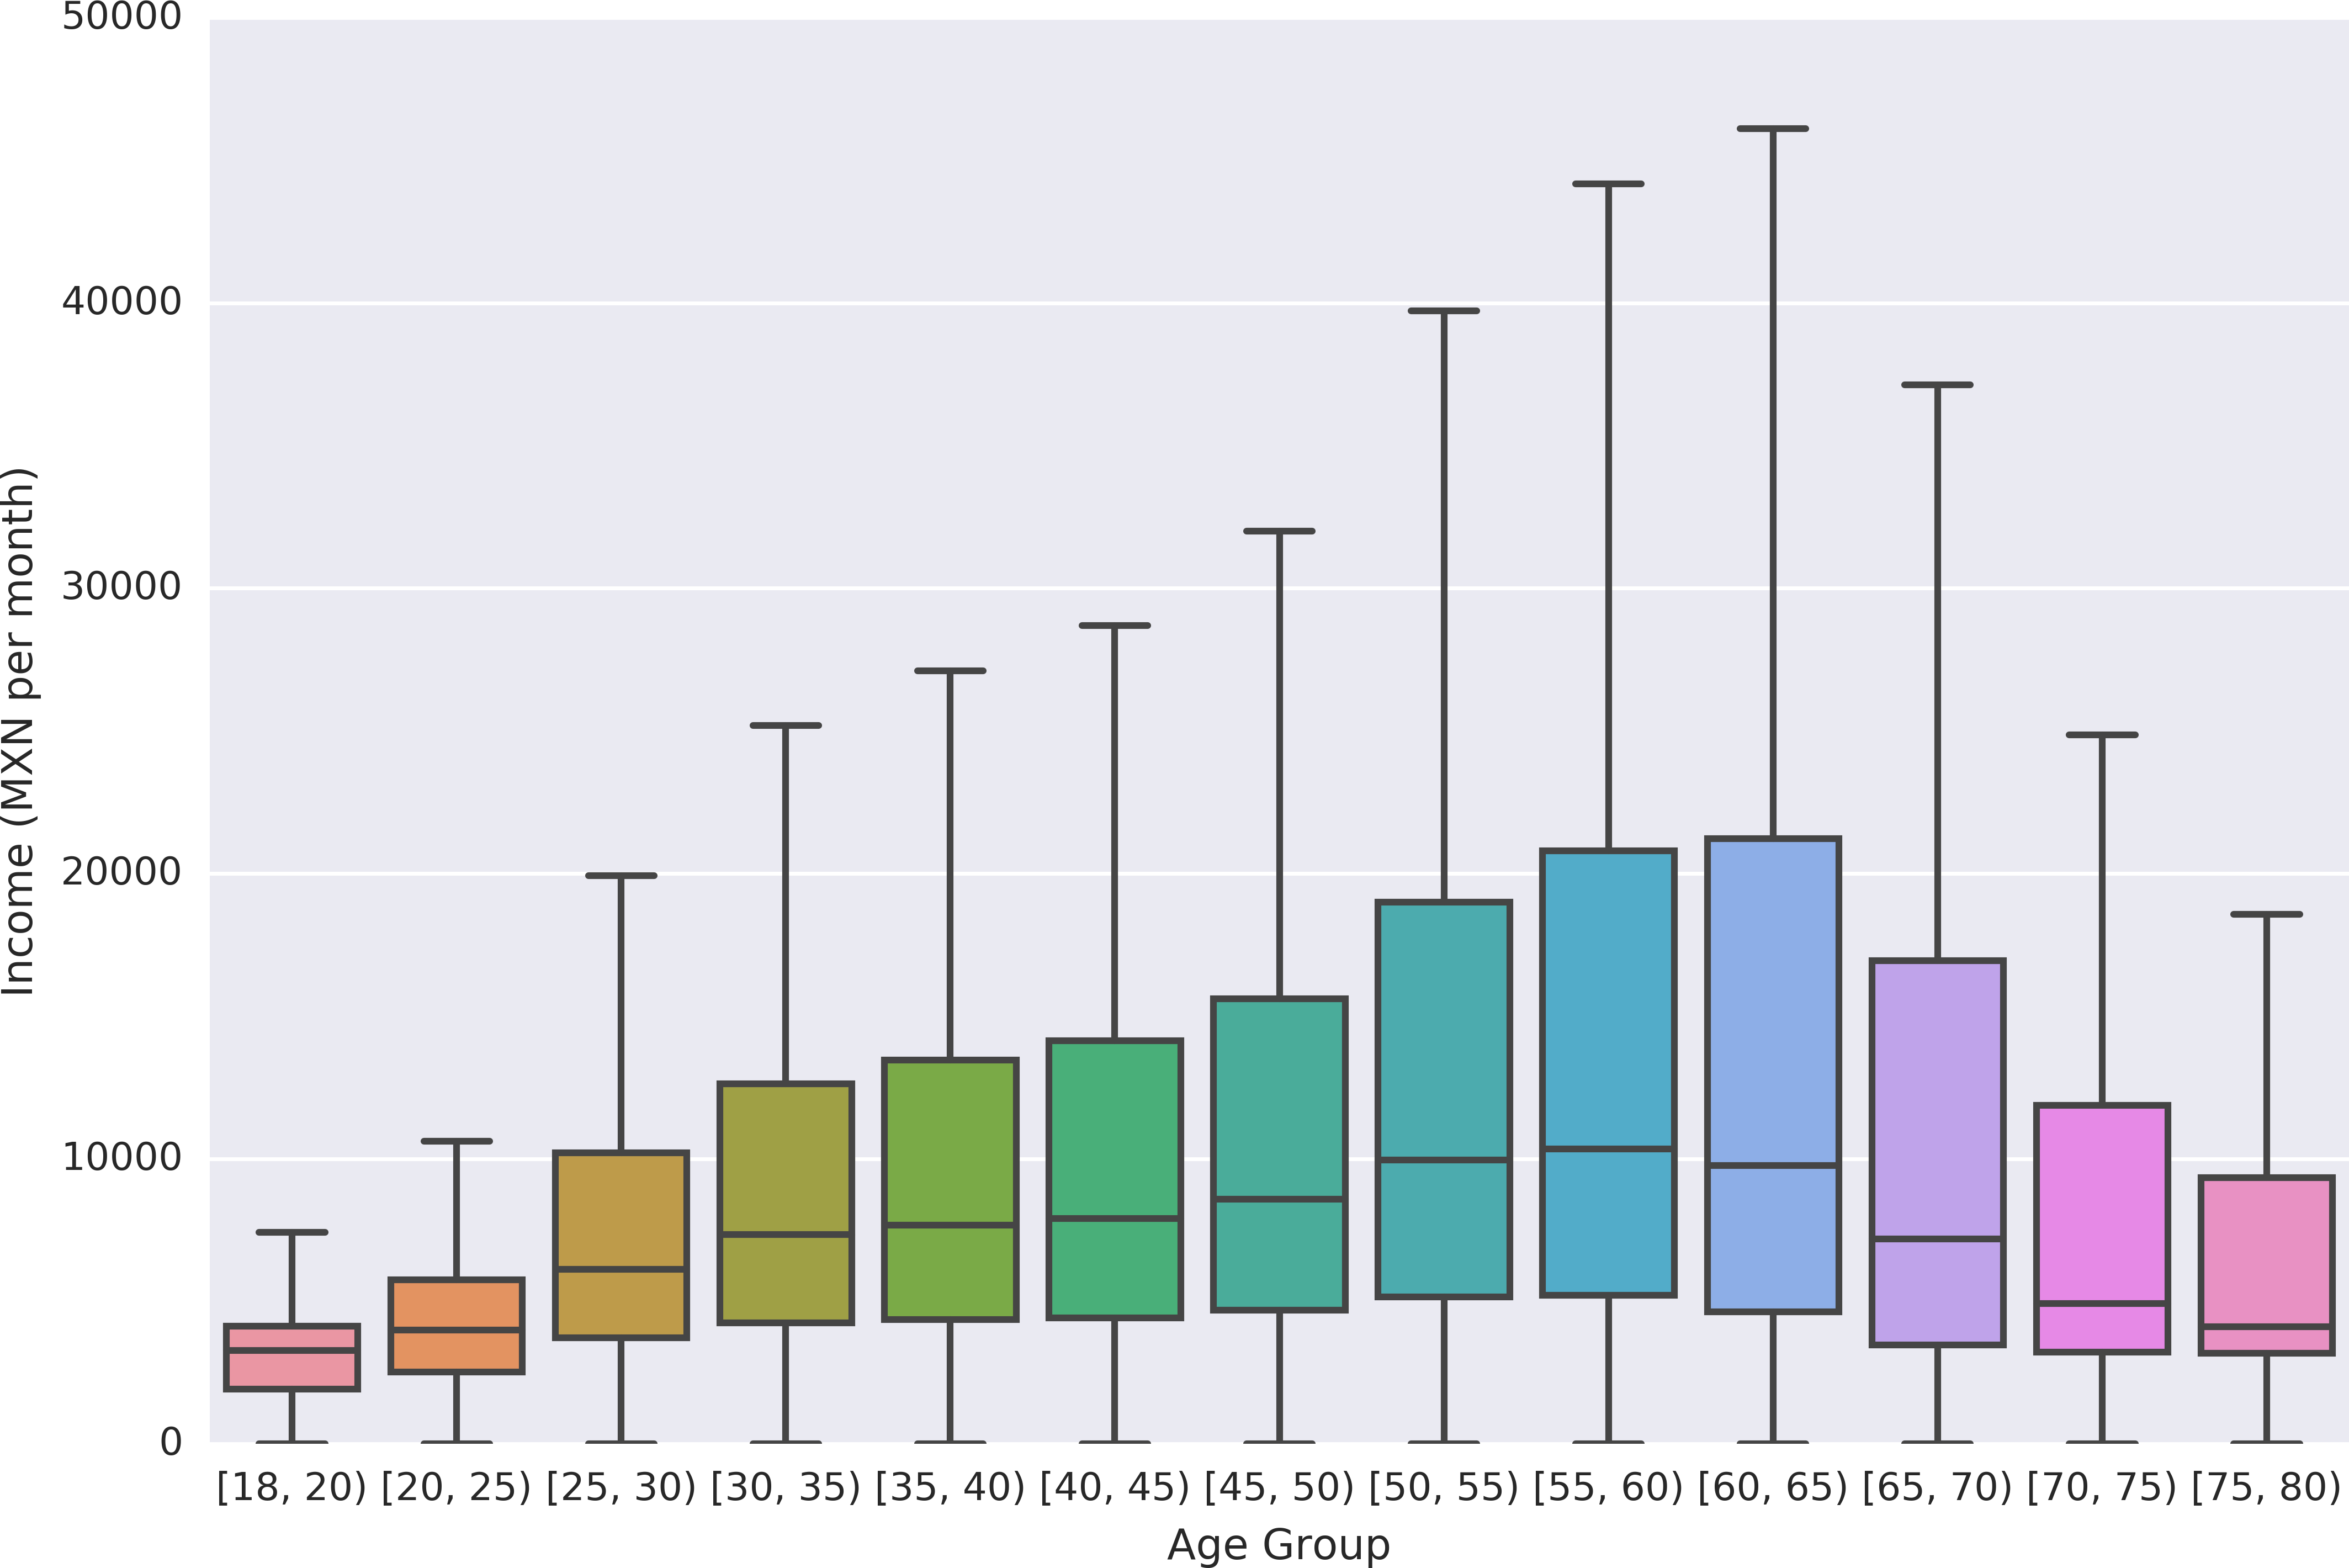
\includegraphics[width=0.9\columnwidth]{figures/income_age_boxplot4/income_age_boxplot4.png}}
\caption{Distribution of income \( b_s \) as a factor of age \( b_a \). This is consistent with data from median house income in Mexico~\cite{gallup2013}.}
\label{income_age_boxplot}
\end{center}
\end{figure}

\Cref{gender_age_bar} shows the distribution of users in \( \mathB \), according to their age range and gender.
\Cref{income_age_boxplot} shows the distribution of income, according to the age range (generated by taking 5 years intervals for the age).
It is interesting to note how the median income increases with the age, up to
the 60--65 years range (the retirement age in Mexico). After 65 years old, the median income rapidly decreases.

\subsection{Bank and Telco Matching}

Since the phone numbers in each call \( p_o \) and \( p_d \) are anonymized with the same hash function as the phone number in the bank data, \( b_p \), we can match users to their unique phone to create the social graph (\( \bowtie \) denotes the inner join operator).

\begin{equation}
G = \mathP \bowtie_{_{p_o = b_p}} \mathB \bowtie_{_{p_d = b_p}} \mathB
\label{join}
\end{equation}

\( G \) includes income information for the subset of the social graph that appears in the bank data, so \( \forall g \in G \) we have its phone number \( g_p \), its average income over 6 months \( g_s \), and its age \( g_a \).
This graph has a total of \num{2027554} nodes with \num{5044976} edges, which represent \num{29599762} calls and \num{5476783} text messages.

\subsection{Outlier Filtering}

The dataset contains information about bank and telco users, some of which may not directly correspond to a human user, % who exclusively users the telco and the bank used in this study,
or may not have useful information for our research.
Most of the telco users in the first case are already filtered by the intersection (\textsc{inner join}). To make sure the users are relevant enough for this study, we only keep the users which have:

\begin{itemize}
	\item More than 5 calls in either direction.
	\item A monthly income of at least \$\num{1000}.
	The value is expressed in Mexican pesos (MXN)\footnote{At the time of writing (July 14, 2016), 1000 Mexican pesos are equivalent to 54 US dollars.}.
	\item A monthly income in the \num{99}th percentile (i.e.\ we filter users with a monthly income in the top 1\%).
\end{itemize}

\subsection{Unequal Distribution of Income}

We provide here some observations of the distribution of income of the bank clients. These observations correspond to the filtered dataset, obtained after applying the filters of the previous section.

\Cref{fig:income_distribution} shows the Lorenz curve, graphical representation of the distribution of income. The X axis plots the cumulative share of clients, ordered from lowest to highest incomes. The Y axis plots the fraction of the total income that they have.

\begin{figure}[ht]
\begin{center}
{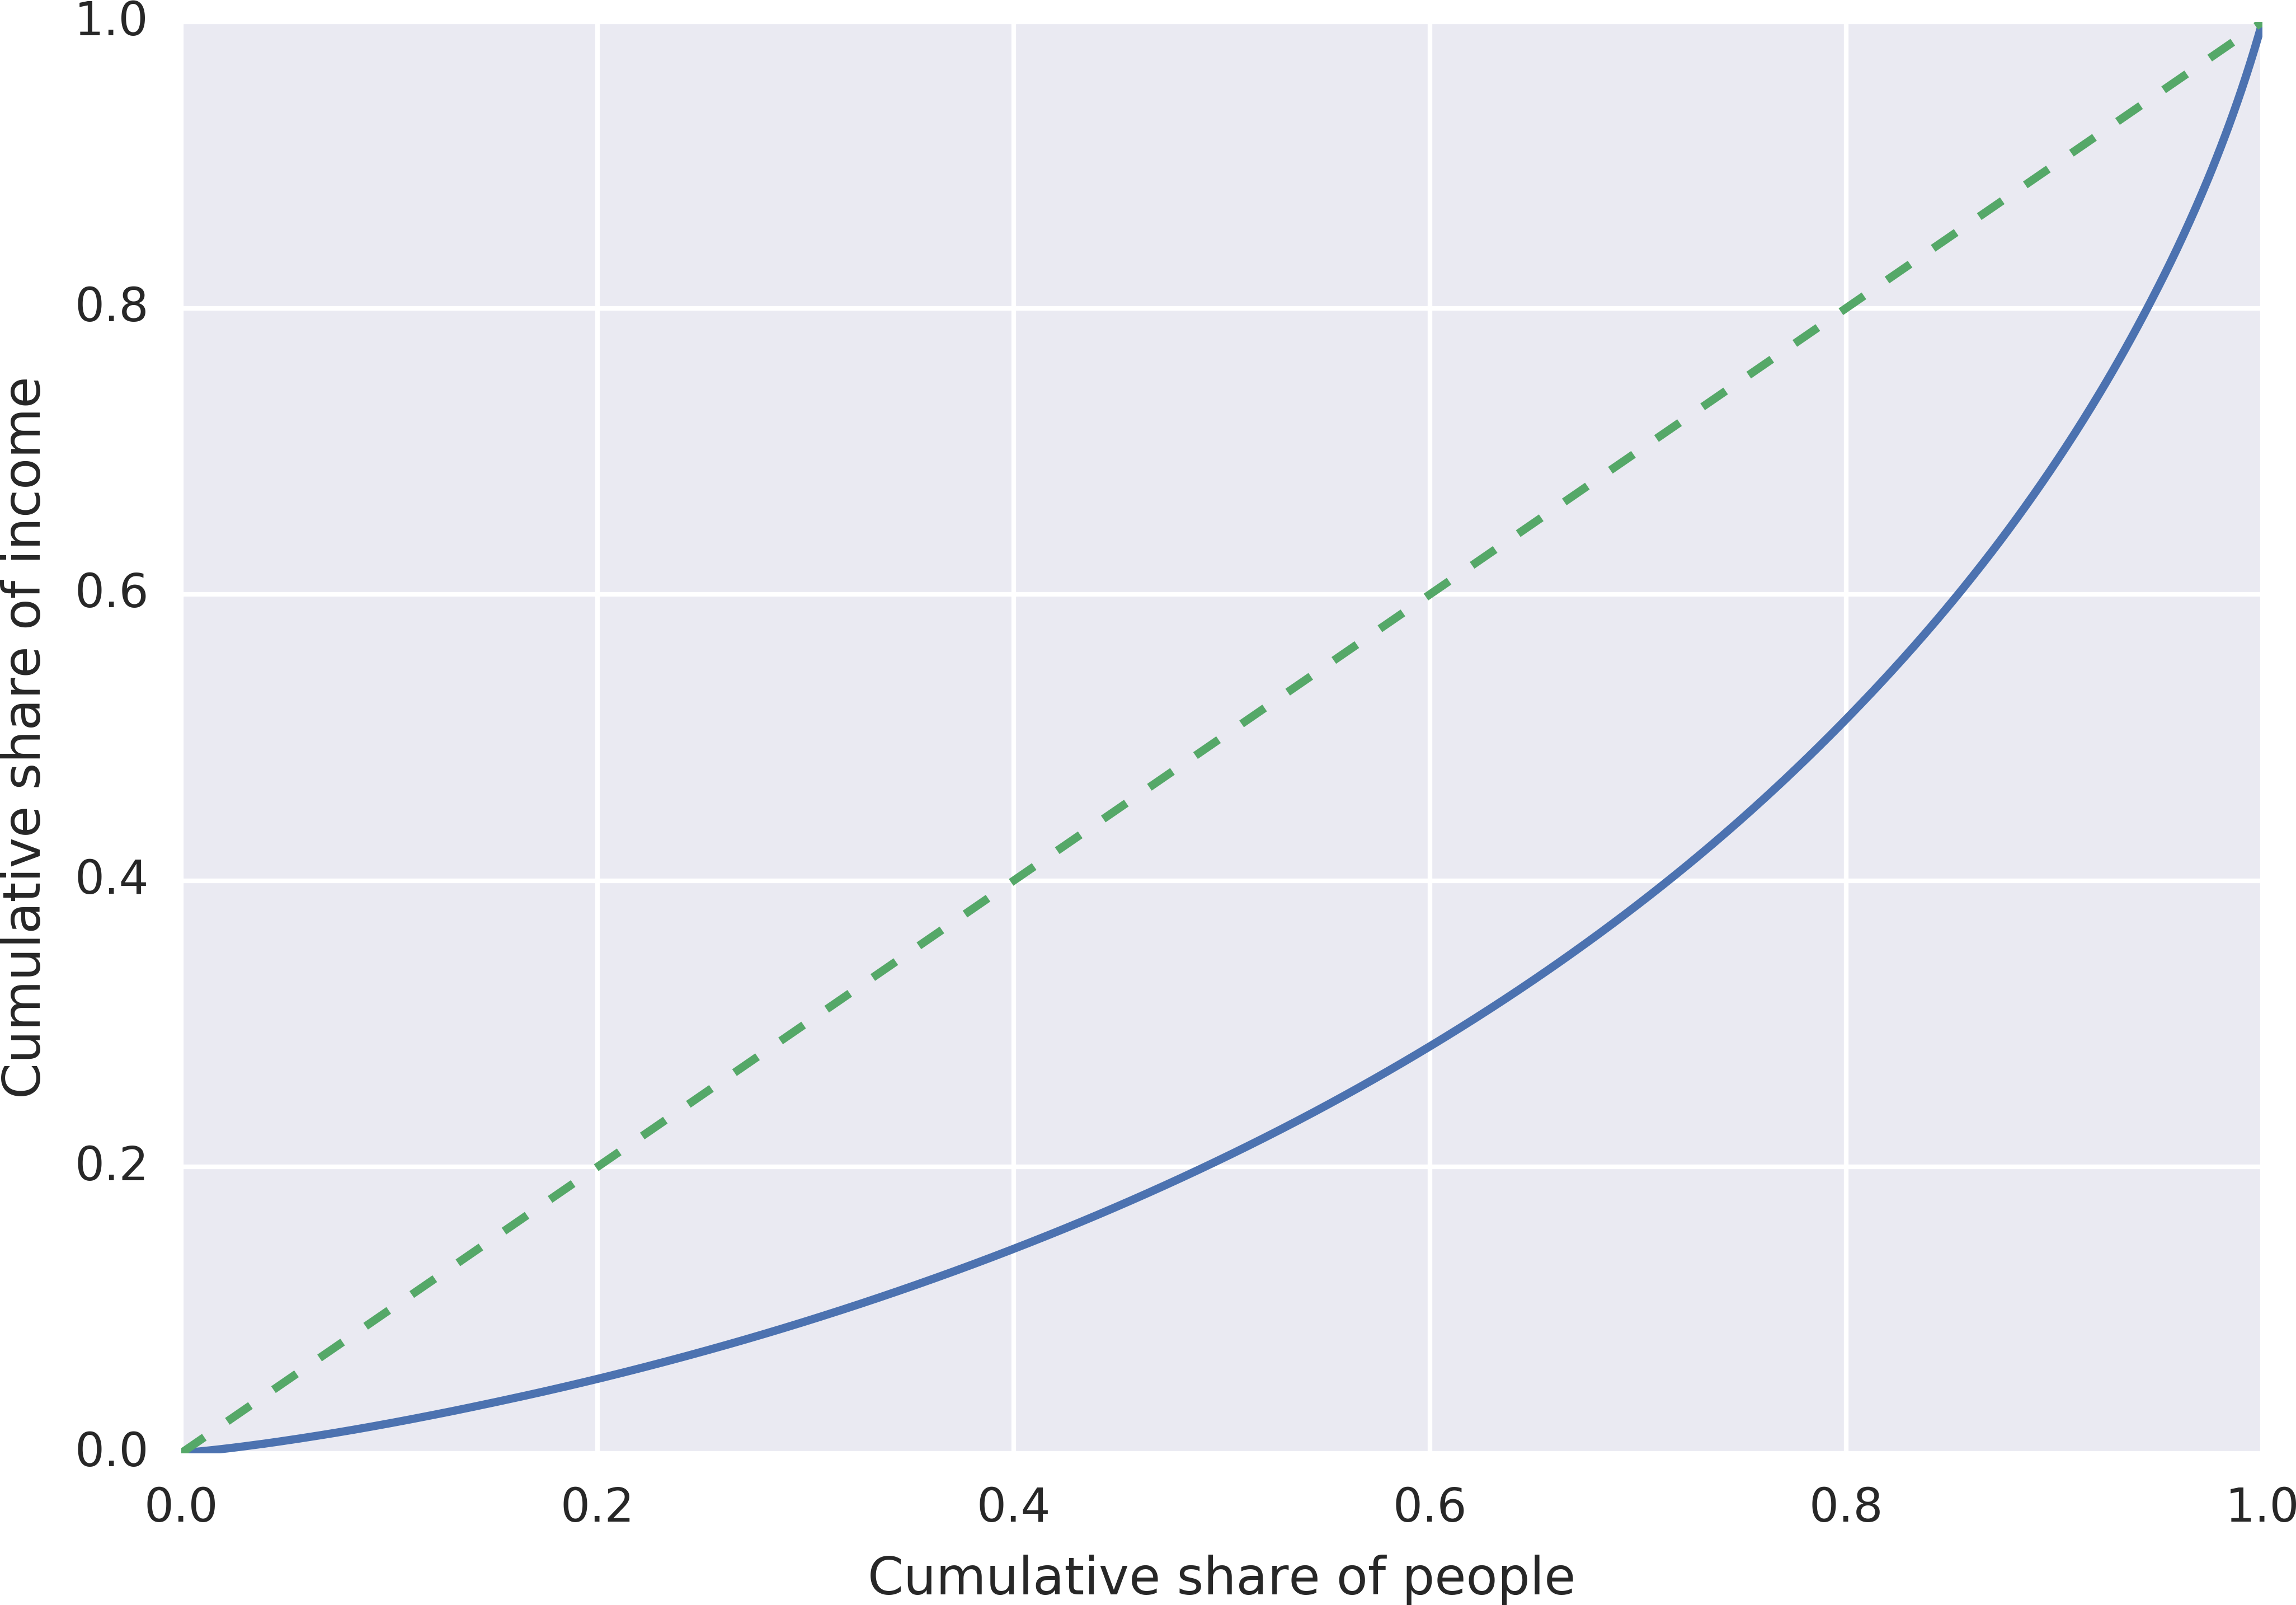
\includegraphics[width=0.9\columnwidth]{figures/cumulative_income.png}}
\caption{Lorenz curve representing the distribution of income of bank clients.}
\label{fig:income_distribution}
\end{center}
\end{figure}

From the Lorenz curve, we can compute the Gini coefficient, as the area that lies between the line of perfect equality (the line at \( 45^{\circ} \)) and the Lorenz curve over the total area under the line of equality.
The Gini coefficient obtained is \( G = 0.45 \).

According to the World Bank~\cite{world_bank}, the Gini coefficient for the whole population of Mexico was 0.481 in 2012. Our result is consistent with this information, since the income inequality is expected to be lower within the bank clients than within the whole population of the country.

Looking at the cumulative share of the clients with highest incomes, we observe that the top 10\% of clients accumulate 33\% of the total income; the top 20\% accumulate 50.5\%; and the top 30\% accumulate 63.1\% of the total income.

% \todo{Distribution per region.}
% \todo{Comparison with statistics from Mexico.}
